\documentclass{amsart}

% for producing the schematic diagram of Figure 1
\usepackage{tikz}

% for bibliography
\usepackage{biblatex}
\addbibresource{proj3bib.bib}

% shortcut macros
\newcommand{\FinA}{F_{1,\textrm{in}}}
\newcommand{\cinA}{c_{1,\textrm{in}}}
\newcommand{\FoutA}{F_{1,\textrm{out}}}

\newcommand{\FinB}{F_{2,\textrm{in}}}
\newcommand{\cinB}{c_{2,\textrm{in}}}
\newcommand{\FoutB}{F_{2,\textrm{out}}}

\begin{document}

\title[Project 3: Pollution in lakes]{
  Math 481, Fall 2024\medskip \\
  Project 3 \\
  Pollution in lakes
}

\author{Gabriel Arteaga}
\address{Department of Mathematics and Statistics\\UMBC\\Baltimore, MD, 21250}
\email{garteag1@umbc.edu}
\date{October 10, 2024}

\begin{abstract}
We present a mathematical model of two interconnected reservoirs and solutes
flowing through them.  We derive a system of differential equation
for the time-dependent concentrations of the solutes in the two
reservoirs.  We apply our model to simulate the concentrations
of pollutants in lakes Erie and Ontario, and investigate the
time that it takes to stabilize the lakes to a lower pollution level
after cutting down the inflow of pollutants.
\end{abstract}

\maketitle

\section{Introduction}
Lake pollution has been an ongoing issue in the Great Lakes for quite some time now. For example in the $1960$'s Lake Erie was officially considered a ``dead lake". Then came the incident of the Cuyahoga River which had previously caught fire numerous times and finally got some attention after \textit{Time} magazine gave it coverage\cite{cuyahoga}. In more recent times run-off from fertilizers plagued Lake Erie with cyanobacterial bloom\cite{erie-pollution}. 
In $1972$ the Clean Water Act was passed and this, for a time, cleaned the Great Lakes tremendously. In this paper, we aim to create a model that can tell us exactly how much acts like the Clean Water Act can positively affect the lakes. More specifically we look at the two reservoir system of Lake Erie and Lake Ontario and analyze how much of an effect they have on the lakes. In Section~\ref{sec:model} we discuss how the two reservoirs model the lakes and define the notation to be used throughout the paper. In Section~\ref{sec:Equations-of-mass} we come up with a system of differential equations to model this general two reservoirs model and proceed to solve it. In Section~\ref{sec:disturbing} we apply the same analysis done in the previous section, but we now implement regulations that decrease each incoming concentration of pollutant by some factors. We then proceed to find equilibrium for this system.  Finally, in this section, we come up with a function that helps us find the efficacy of these regulations. In Section~\ref{sec:Lake-Erie-Ontario} we assign our regulation factors numerical values and then analyze the results of our function when they reach our wanted efficacy. Finally in Section~\ref{sec:effect} we look at the ratio of our equilibrium concentrations to evaluate how effective our regulations have been. 




\section{The model}\label{sec:model}

The schematic diagram in Figure~\ref{fig:schematic_diagram}
represents two interconnected and well-stirred reservoirs
of volumes $V_1$ and $V_2$.  A solute of concentration
$\cinA$ enters the first reservoir at the volumetric flow rate
of $\FinA$.  The output of the first reservoir flows into
the second reservoir where it joins another inflow of the
same solute at concentration $\cinB$ at the flow rate of
$\FinB$, then the mixture flows out at the rate of~$\FoutB$.
The concentrations of the solutes in the two reservoirs are
$c_1(t)$ and~$c_2(t)$.

In this case study we will assume that the volumes $V_1$ and $V_2$,
the flow rates $\FinA$ and $\FinB$, and the input concentrations
$\cinA$ and $\cinB$ are constants, that is, they
they do not change with time.  Consequently, $\FoutA = \FinA$ and
$\FoutB = \FoutA + \FinB$.

\begin{figure}
  \centering
  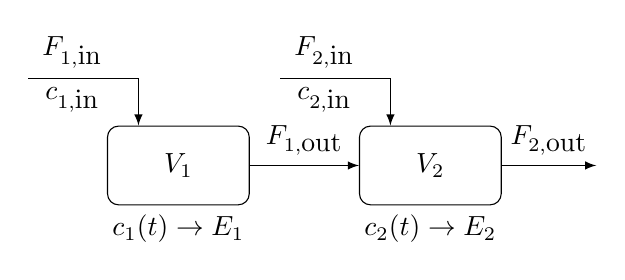
\begin{tikzpicture}[>=latex]
    \tikzstyle{boxed}=[draw=black, minimum width=1.8cm, minimum height=1cm,
      rounded corners]
    \draw (0,0)   node[boxed, label=below:$c_1(t) \to E_1$] (V1) {$V_1$};
    \draw (3.2,0) node[boxed, label=below:$c_2(t) \to E_2$] (V2) {$V_2$};
    \draw[->] (V1.east) -- node[above] {$\FoutA$} (V2.west);
    \draw[->] (V2.east) -- node[above] {$\FoutB$} +(1.2,0);
	\draw[<-] (node cs:name=V1, angle=135) |- +(-1.4,0.6)
		node[above, pos=0.8] {$\FinA$}
		node[below, pos=0.8] {$\cinA$};
	\draw[<-] (node cs:name=V2, angle=135) |- +(-1.4,0.6)
		node[above, pos=0.8] {$\FinB$}
		node[below, pos=0.8] {$\cinB$};
  \end{tikzpicture}
  \caption{A schematic diagram of two interconnected reservoirs.
     If the volumes $V_1$ and $V_2$, the flow rates $\FinA$ and $\FinB$,
     and the input concentrations $\cinA$ and $\cinB$ are constants, then
     the concentrations $c_1(t)$ and $c_2(t)$ in the reservoirs
     tend to equilibrium values $E_1$ and $E_2$
     in the long term.}
  \label{fig:schematic_diagram}
\end{figure}

\section{The equations of balance of mass}\label{sec:Equations-of-mass}
First let's analyze the behavior of a single reservoir, that being Lake Erie, using our description of the system from section~\ref{sec:model} we find that we have one input and one output which correlate to the rate of change of volume and concentration. As such we find that the differential equation of pollutants for a single reservoir comes to 
\[
    \frac{dVc(t)}{dt}=F(c_{in})-Fc(t).
\]

Note that in our complete system, we will have two reservoirs. Our equation for the first reservoir stays relatively the same. However, for our second, we need to consider now additional flow rate input this comes out to 
\[
    \frac{dV_2c(t)}{dt}=\FinB\cinB+\FinA c_1(t)-\FoutB c_2(t).
\]
We use our definitions from section~\ref{sec:model} we arrive to

\[
 \frac{dV_2c(t)}{dt}=(\FoutB -\FinA)\cinB+\FinA c_1(t)-\FoutB c_2(t).
\]
Factoring we arrive at the equation
\[
    \frac{dV_2c(t)}{dt}=\FinA (c_1(t)-\cinB)+\FoutB( \cinB-c_2(t)).
\]
Now we construct our system
\begin{equation*}
    \left\{
    \begin{aligned}
        &\frac{dV_1c_1(t)}{dt}=\FinA(\cinA-c_1(t)),\\
        &\frac{dV_2c_2(t)}{dt}=\FinA (c_1(t)-\cinB)+\FoutB(\cinB-c_2(t)).
    \end{aligned}
    \right.
\end{equation*}
Recall that our volumes are constant so we re-write to 
\begin{equation*}
    \left\{
    \begin{aligned}
        &\frac{dc_1(t)}{dt}=\frac{\FinA}{V_1}(\cinA-c_1(t)),\\
        &\frac{dc_2(t)}{dt}=\frac{\FinA }{V_2}(c_1(t)-\cinB)+\frac{\FoutB}{V_2}(\cinB-c_2(t)).
    \end{aligned}
    \right.
\end{equation*}
Now that we have our system for $c_1(t)$ and $c_2(t)$ we need to discuss the topic of retention time. Retention time, which in this paper we define as $\tau$, is how long it takes for a particle to travel through a body of water. Including this in our system simplifies it as,
\[
    \tau=\frac{F}{V},
\]
or
\[
    \frac{1}{\tau}=\frac{V}{F}.
\]
Note that this fraction appears numerous times throughout our system. As such we rewrite 
\begin{equation*}
    \left\{
    \begin{aligned}
        &\frac{dc_1(t)}{dt}=\frac{1}{\tau_1}(\cinA-c_1(t)),\\
        &\frac{dc_2(t)}{dt}=\frac{\FinA }{V_2}(c_1(t)-\cinB)+\frac{1}{\tau_2}(\cinB- c_2(t)).
    \end{aligned}
    \right.
\end{equation*}
However, we are still troubled with one term that uses flow rate. Note that we can express
\[
    \frac{\FinA}{V_2}=\left(\frac{\FinA}{V_1}\right)\left(\frac{V_1}{V_2}\right)=\frac{V_1}{V_2\tau_1}.
\]
Using this definition we can finally come to 
\begin{equation*}
    \left\{
    \begin{aligned}
        &\frac{dc_1(t)}{dt}=\frac{1}{\tau_1}(\cinA-c_1(t)),\\
        &\frac{dc_2(t)}{dt}=\frac{V_1}{V_2\tau_1}(c_1(t)-\cinB)+\frac{1}{\tau_2}(\cinB- c_2(t)).
    \end{aligned}
    \right.
\end{equation*}
We define some initial values with this system, which will stay arbitrary for now. These are
\[
c_1(0)=c_{1,0}, c_2(0)=c_{2,0},
\]
and these ultimately bring our system to be, 
\begin{equation}\label{eq:system}
    \left\{
    \begin{aligned}
        &\frac{dc_1(t)}{dt}=\frac{1}{\tau_1}(\cinA-c_1(t)),c_1(0)=c_{1,0},\\
        &\frac{dc_2(t)}{dt}=\frac{V_1}{V_2\tau_1}(c_1(t)-\cinB)+\frac{1}{\tau_2}(\cinB- c_2(t)), c_2(0)=c_{2,0}.
    \end{aligned}
    \right.
\end{equation}

We now solve this system to get our solutions,
\begin{subequations}
  \begin{align}
    c_1(t)&=e^{-\frac{t}{\tau_1}}(c_{1,0}-\cinA)+\cinA\label{eq:c1sol},\\
    c_2(t)&=c_{1,0}\left(\frac{\tau_2 V_1 \left( e^{-\frac{t}{\tau_1}} - e^{-\frac{t}{\tau_2}} \right)}{(\tau_1 - \tau_2) V_2}\right)+c_{2,0}e^{-\frac{t}{\tau_2}}\label{c2sol}\\
    &\qquad+\cinA\left(\frac{V_1 \tau_2 \left( e^{-\frac{t}{\tau_1}} \tau_1 - e^{-\frac{t}{\tau_2}} \tau_2 - \tau_1 + \tau_2 \right)}{(\tau_1 - \tau_2) \tau_1 V_2}\right)\notag\\
    &\qquad-\cinB\left(\frac{\left( e^{-\frac{t}{\tau_2}} - 1 \right) (\tau_1 V_2 - \tau_2 V_1)}{\tau_1 V_2}\right)\notag
  \end{align}  
\end{subequations}


We now move on to finding the equilibrium states of this system, we will call these $E_1$ and $E_2$ respectively. We note that after a long period, the concentration of each reservoir will reach equilibrium with the water entering. For that, we will take the limit of each function
\begin{align*}
    &E_1=\lim_{x \to \infty}c_1(t)= \cinA,\\
    &E_2=\lim_{x \to \infty}c_1(t)=\frac{\tau_2V_1\cinA}{\tau_1V_2}+\cinB\left(1-\frac{\tau_2V_1}{T_1V_2}\right).
\end{align*}

\section{Disturbing the system} \label{sec:disturbing}
Suppose we impose regulations that decrease the concentration of pollutants in the incoming water in each system. This means that the incoming pollutants, $\cinA$ and $\cinB$, will be scaled down by factors of what we will call $\alpha$ and $\beta$. We also assume that we are starting from equilibrium, or $E_1, E_2$ from section~\ref{sec:model}. We replace each $\cinA$ and $\cinB$ in our system~\ref{eq:system} with $\alpha\cinA$ and $\beta\cinB$ respectively to account for regulations. This gives us, 

\begin{equation*}\label{eq:disturbed-sys}
    \left\{
    \begin{aligned}
        &\frac{dc_1(t)}{dt}=\frac{1}{\tau_1}(\alpha\cinA-c_1(t)),c_1(0)=E_1,\\
        &\frac{dc_2(t)}{dt}=\frac{V_1}{V_2\tau_1}(c_1(t)-\beta\cinB)+\frac{1}{\tau_2}(\beta\cinB- c_2(t)),c_2(0)=E_2.
    \end{aligned}
    \right.
\end{equation*}
We again look for solutions to this system and arrive at
\begin{subequations}
  \begin{align}
    c_1(t)&=\left( (\alpha - 1) e^{-\frac{t}{\tau_1}} - \alpha \right) c_1,\label{eq:disturbedc1}\\
    c_2(t)&=-\cinA\left(\frac{\tau_2 \left( \tau_1 (\alpha - 1) e^{-\frac{t}{\tau_1}} - \tau_2 (\alpha - 1) e^{-\frac{t}{\tau_2}} - \alpha (\tau_1 - \tau_2) \right) V_1 }{(\tau_1 - \tau_2) \tau_1 V_2}\right)\label{eq:disturbedc2}\\
    &\qquad-\cinB\left(\frac{(\tau_1 V_2 - \tau_2 V_1) \left( (\beta - 1) e^{-\frac{t}{\tau_2}} - \beta \right) }{\tau_1 V_2}\right).\notag
  \end{align}  
\end{subequations}
We once again look for equilibrium states, so we take limits. For this equilibrium, we will call them $e_1$ and $e_2$ respectively, 
\begin{align}
    &e_1=\alpha\cinA,\\
    &e_2=\frac{\alpha\tau_2V_1\cinA}{\tau_1V_2}+\cinB\left(\beta-\beta\frac{\tau_2V_1}{T_1V_2}\right).
\end{align}
We now want to see how long it will ultimately take for $c_1(t)$ and $c_2(t)$ to come to a relative notion of equilibrium. We look at this by taking the difference of $c_2(t)$ and $e_2$, note we only look at the difference for $c_2(t)$ as it is the final reservoir we are analyzing. We denote this difference by 
\begin{equation*}\label{eq:delta}
\begin{aligned}
	\delta(t)=c_2(t)-e_2.
\end{aligned}
\end{equation*}
However hoping that this number goes to zero will take quite a long time, so we accept some small margin of pollutants. We define acceptable efficacy at $5\%$ of $e_2$. This percentage was chosen arbitrarily, this can be adjusted to other acceptable levels of efficacy. This gives us efficacy at, 
\[\delta(t)=(.05)e_2,\]
or
\[\frac{\delta(t)}{e_2}=0.5.\]
Note that this is still a function of time, as such we can still graph this, and rather than solving for delta to get to $5\%$ of $e_2$ we solve for when the function, which we will call $p(t)$ achieves $.5$. So we define, 
\begin{equation*}
\begin{aligned}
p(t)=\frac{\delta(t)}{e_2}.
\end{aligned}
\end{equation*}
However, if we attempt to use this ratio we will run into some issues, that being that we do not know the specific values of $\cinA$ and $\cinB$. Rather than looking at these individually, we will look at their ratio, as we know that Erie is more polluted than Ontario and thus the ratio will be less than one. Thus we define, 
\[
	R=\frac{\cinB}{\cinA}.
\]
To make the equation of $p(t)$ easier to work with we will substitute $\cinB$ with $R\cinA$. Now rather than using this symbolically we will use the real-world numbers for values like retention time and volume. That gives us
\begin{align}
V_1=395 \text{ mi}^3, V_2=119 \text{ mi}^3, \tau_1=6 \text{ years}, \tau_2=2.6 \text{ years}.
\end{align}
Note these numbers appear from~\cite{erie-vol,ontario-vol-retention,erie-retention}. We now calculate an expression for $p(t)$, note we limit significant figures to three decimals. That is, 
\begin{equation*}\label{eq:p-withvals}
\begin{aligned}
p(t)=\frac{\left( -0.230 \, \alpha + 0.230 \right) e^{-\frac{t}{6}} + \left( 0.0998 \, \alpha - 0.0998 + \left( -0.869 \, \beta + 0.869 \right) R \right) e^{-0.385 t}}{0.131 \, \alpha + 0.869 \, \beta \, R}.
\end{aligned}
\end{equation*}
\section{Lakes Erie and Ontario}\label{sec:Lake-Erie-Ontario}

Suppose now that we consider a set of stringent regulations, such that we reduce by factors of one-half for Lake Erie ($\alpha=\frac{1}{2}$), and one-fourth for Lake Ontario ($\beta=\frac{1}{4}$). Using equation~\ref{eq:p-withvals} from earlier we get, 
\begin{equation*}\label{eq:p-withab}
\begin{aligned}
p(t)=\frac{-0.257 e^{-0.385t} + 0.594 e^{-0.167t} + 0.242 e^{-0.167t} R}{0.337 + 0.0815 R}.
\end{aligned}
\end{equation*}
Note that we still have values of $R$ left in this expression. To address this recall what was mentioned in section~\ref{sec:disturbing}, that being that $R$ will always be less than one. So to account for this when we calculate we will take several values of $R$, those being $0.3,0.5,0.7$. We show the graphs of all three in Figure~\ref{fig:pgraph}.
\begin{figure}\label{fig:pgraph}
    \centering
    \includegraphics[width=0.8\linewidth]{pgraph.png}
    \caption{The line in red represents $p(t)$ with an $R$ value of $0.3$, the line in blue represents $p(t)$ with an $R$ value of $0.5$, and the line in green represents $p(t)$ with an $R$ value of $0.7$.}
    \label{fig:enter-label}
\end{figure}
From this, we can obtain when our model will come to $5\%$ of $e_2$. For each value of $R$ we see that for a value of $0.3$ we reach $5\%$ at roughly $21.637$ years, for $0.5$ it is $21.798$ years, and for $0.7$ it is $21.941$ years. Ultimately we reach an average of $21.792$ years until we reach our accepted level of efficacy. 




\section{The effect of the cleanup}\label{sec:effect}
Now we aim to see exactly how effective these regulations have been. To do so we analyze the ratio of our new equilibrium, $e_2$, and our old equilibrium, $E_2$. That expression comes out to, 
\begin{equation*}
\begin{aligned}
\frac{e_2}{E_2}=\frac{\beta R \left( \tau_1 V_2 - \tau_2 V_1 \right) + \alpha \tau_2 V_1}{V_1 \tau_2 + \left( \tau_1 V_2 - \tau_2 V_1 \right) R}.
\end{aligned}
\end{equation*}
Recalling our parameters from section~\ref{sec:disturbing}, it becomes,
\begin{equation*}\label{eq:equil-rat}
\begin{aligned}
\frac{e_2}{E_2}=\frac{82.975 R + 345.600}{691.200 + 331.900 R}.
\end{aligned}
\end{equation*}
However, we run into the same issue as before where we must take $R$ to be differing values all less than one. For an $R$ value of $.3$, we come to, $.469$. For an $R$ of $0.5$, we come to, $.452$. Finally, for an $R$ of $.07$, we come to $.437$. This gives us an average of $0.452$. Thus we can conclude that our regulations have been effective, as we are only left with $.452$ of our starting equilibrium. 

\section{Conclusion}
In this paper, we have created a model that lets us detect changes in the concentration of pollutants in Lake Erie, and Lake Ontario. By analyzing a system of differential equations based on the inflow and outflow rates of a two-reservoir system, and using lake volumes and residence times, we found the time it takes for our model to reach efficacy. Ultimately this told us how effective our regulations were at decreasing pollutant levels. 





\printbibliography

\end{document}
